\begin{figure*}[!t]
    \centering
    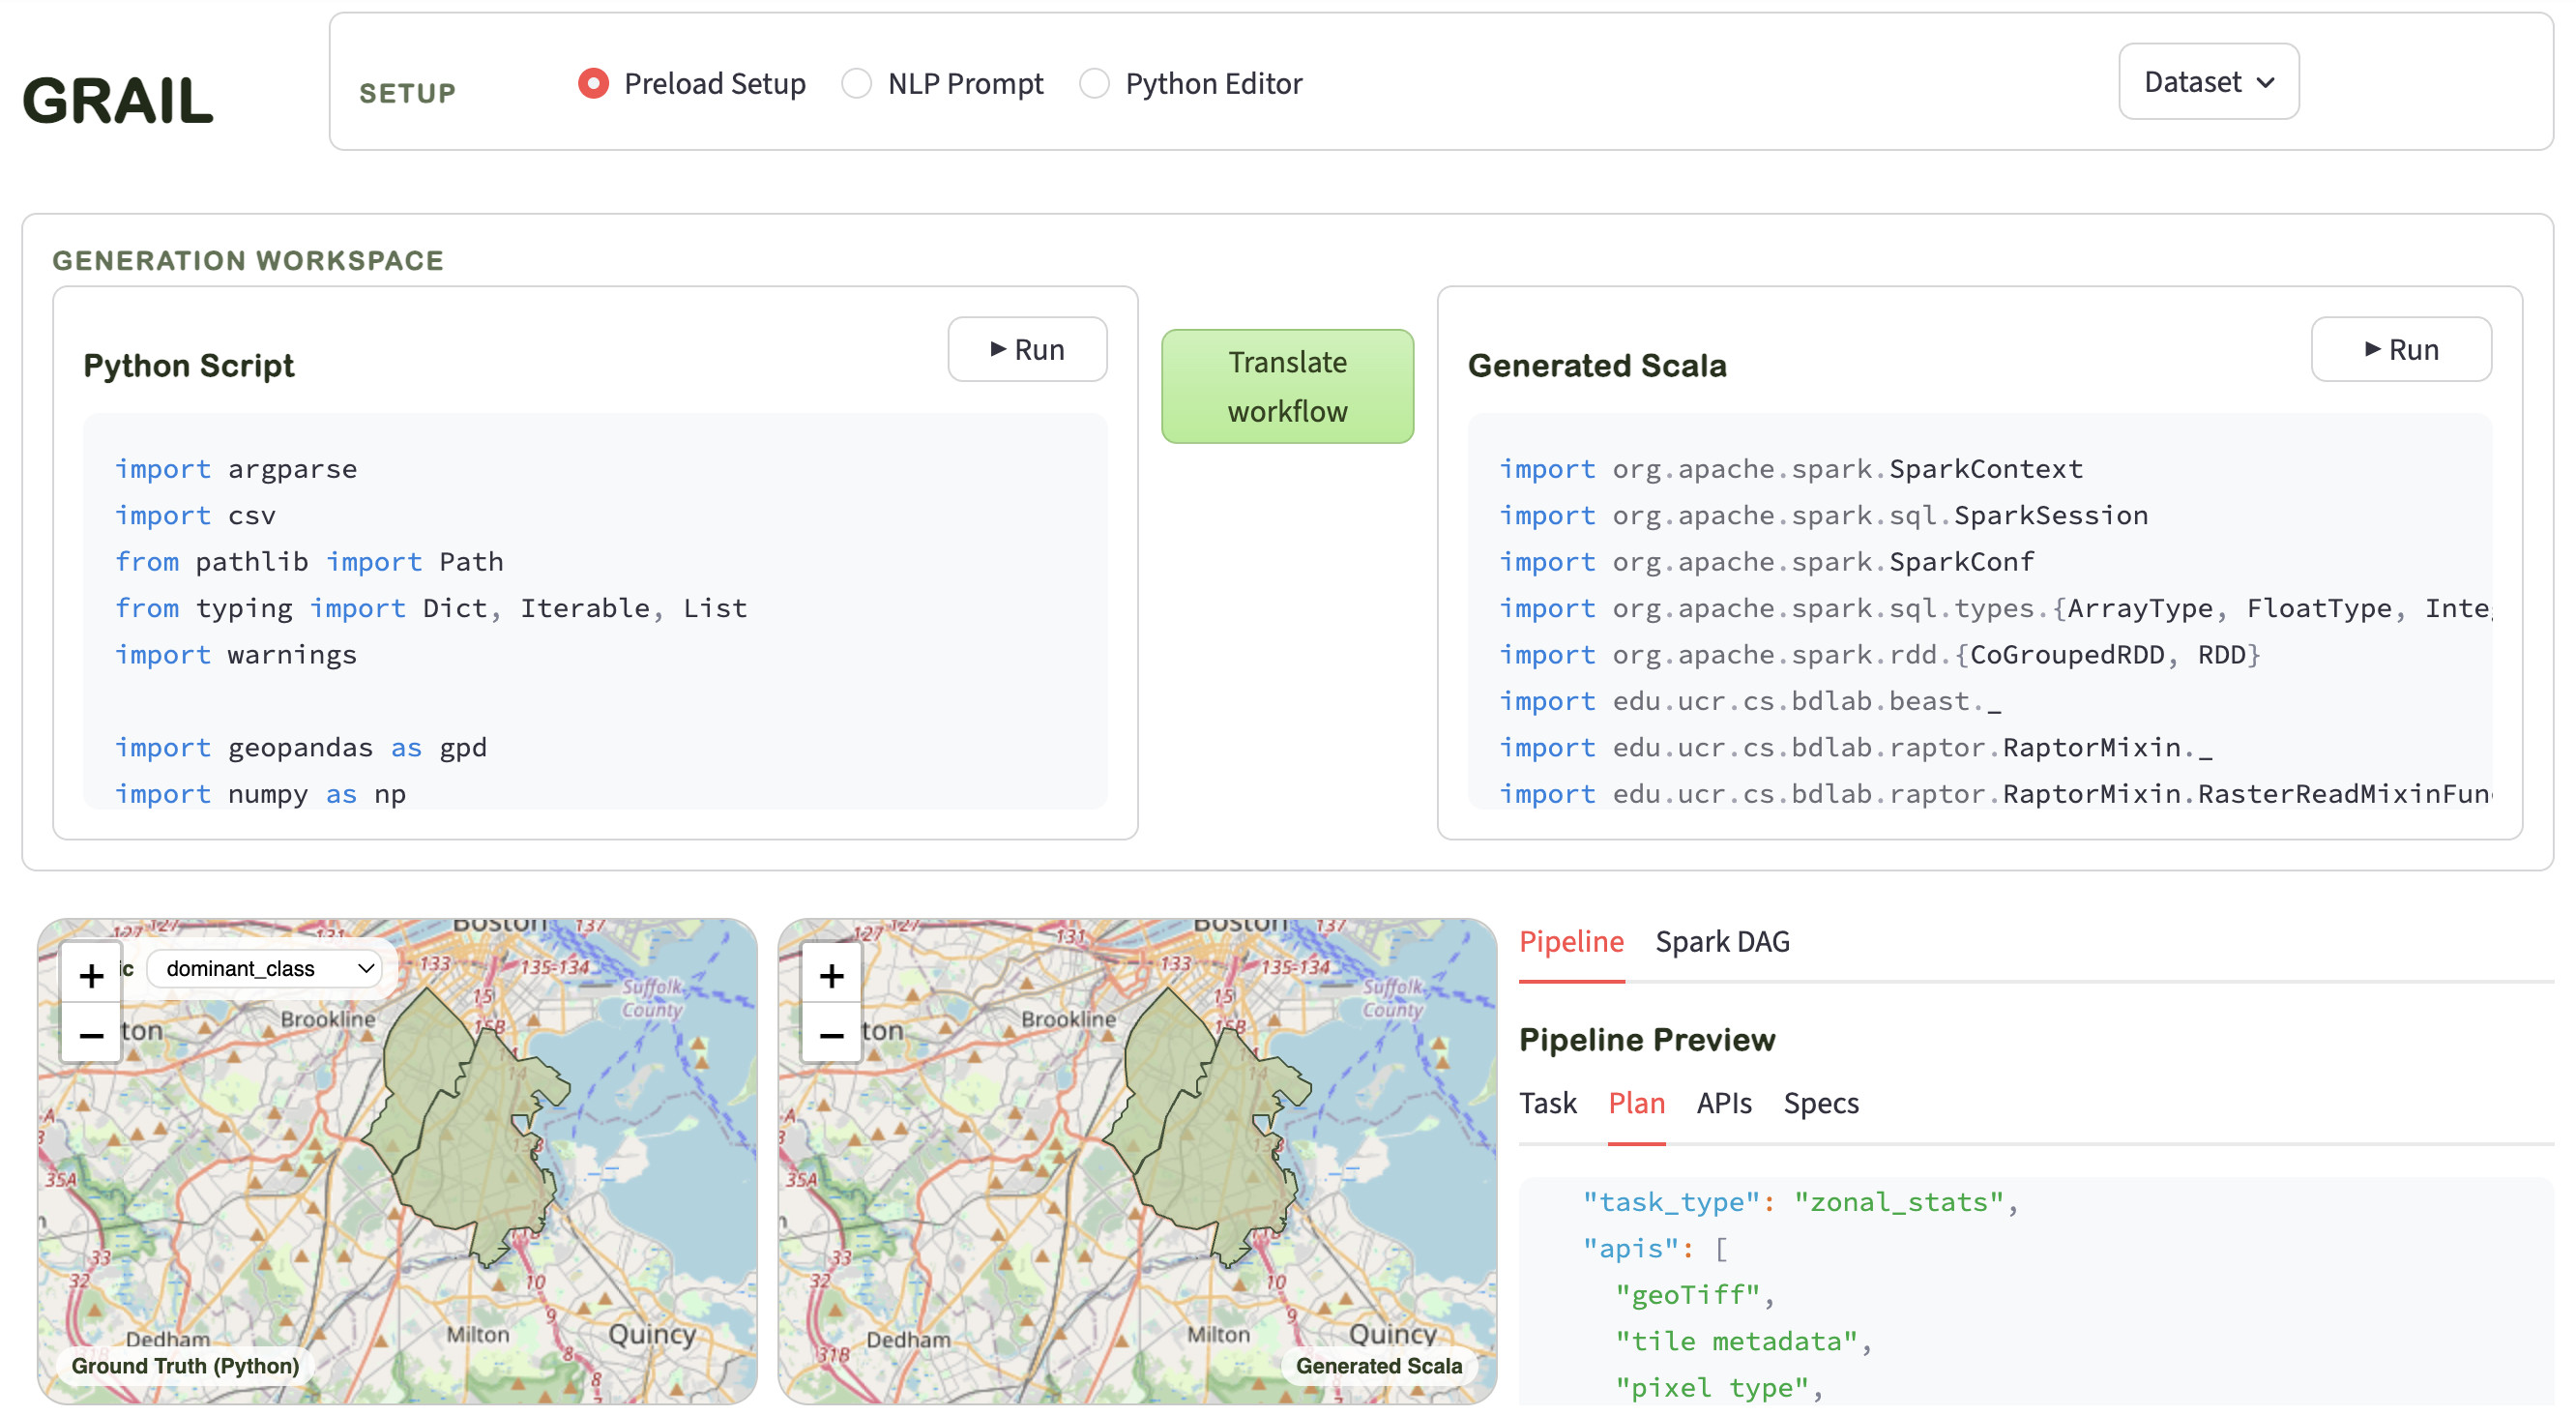
\includegraphics[width=0.85\textwidth]{figures/interface.png}
    \caption{User Interface of GRAIL.}
    \label{fig:interface}
\end{figure*}
\section{Demo Scenarios}
\label{sec:demo}
% Figure A: code translation side-by-side
% Figure B: map + pipeline preview
% \begin{figure}[H]
%     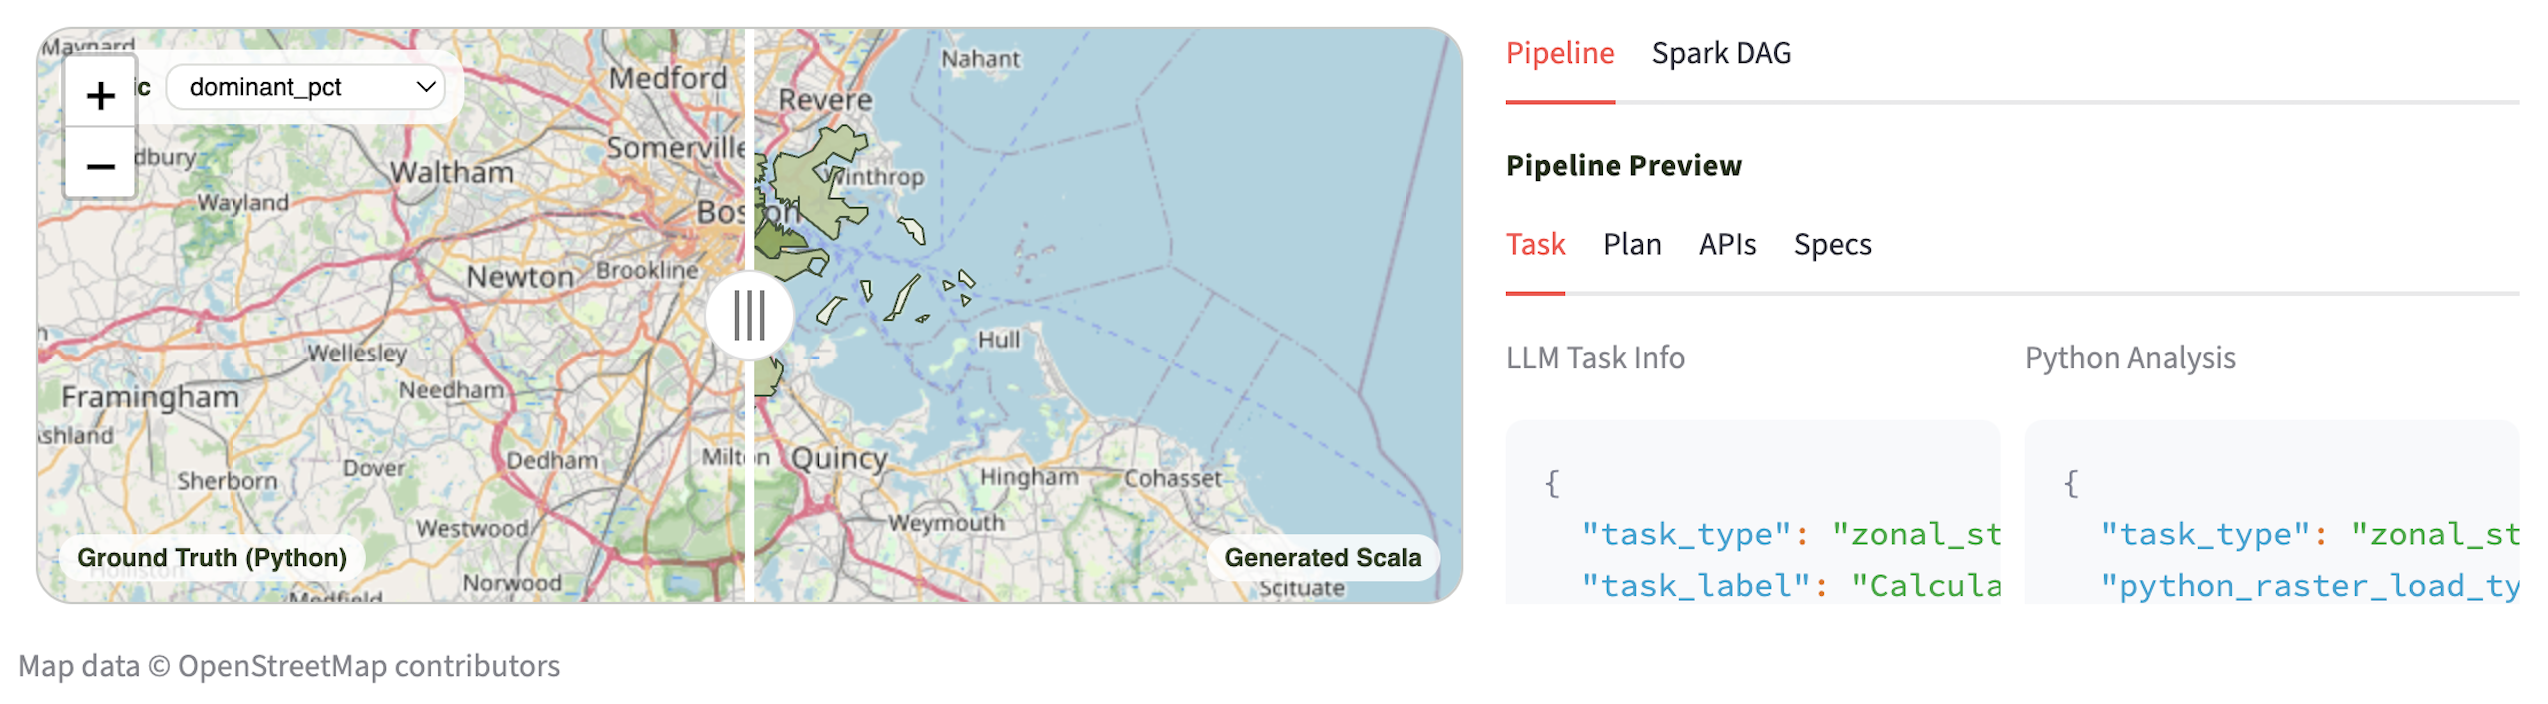
\includegraphics[width=\columnwidth]{figures/interface_2.png}
%     \caption{Split-view result map and Pipeline Preview panel.}
%     \label{fig:interface_2}
% \end{figure}
\subsection{Boston Land Use: Translating Python to RDPro Scala}
In this demo scenario, we walk through a representative use case 
using our GRAIL interface. The user uploads a Python script that 
computes the percentage of each land use type across cities in 
the Boston area. %While functional on a single machine, the 
%original Python script does not scale to large raster datasets or 
%complex geometries. RDPro Scala addresses this by distributing 
%computation across a cluster.
As shown in Figure~\ref{fig:interface}, the interface presents 
the original Python script on the left alongside the generated Scala 
code on the right, produced by GRAIL translation pipeline. 
Bottom part of the figure shows the result comparison in a split map view, where 
users can inspect the Python and Scala outputs side by side to verify 
correctness. Users can also examine the pipeline steps selected by 
the agent and the Spark DAG generated during distributed execution. Our platform also supports plain-text translation and raw Python script editing using the setup panel at the top. Users also have the free choice of choosing a different dataset or using the pre-loaded one for experience.

%input Boston shapefile
%Land use national wide
%return for each city the main landuse type
% the Spark DAG
% the result comparasion 
In this experiment, we use two cities, Roxbury and Dorchester, as sample study areas. The NLCD dataset is cropped with a spatial extent larger than the bounding boxes of these two cities to ensure full coverage during spatial operations. Figure~\ref{fig:nlcd} presents a split-view comparison, the left image shows the ground truth result produced using Python, while the right image shows the output generated by the GRAIL Scala code. Both results consistently indicate that the dominant land use class is label 23, corresponding to Developed, Medium Intensity.
%Furthermore, Figure~\ref{fig:dag} illustrates the Spark job execution and its corresponding DAG for the spatial join between the NLCD raster and the Boston shapefile. This visualization enables users to inspect whether the LLM-generated Scala code produces a reasonable and efficient execution plan.
\begin{figure}[t]
    \centering
    
\includegraphics[width=0.85\columnwidth]{figures/boston.png}
    \caption{Comparison of dominant land use classification for Roxbury and Dorchester. 
Left: ground truth generated using Python. Right: result produced by LLM-generated Scala code.}
    \label{fig:nlcd}
\end{figure}

% \begin{figure}[H]
%     
\includegraphics[width=\columnwidth]{figures/dag.png}
%     \caption{Spark execution DAG for the spatial join between the NLCD raster and the Boston shapefile.}
%     \label{fig:dag}
% \end{figure}
